\chapter{Correzione ottiche}
\textit{Riferimento pag 109-110 manuale}
\\\\
Le lettere sono figure percepite dall'occhio e la loro forma, di conseguenza, \hl{deve seguire un rigore ottico, piuttosto che geometrico}. Infatti, se si seguisse la pura geometria, le lettere risulterebbero squilibrate, sbilanciate e poco armoniose.

Entrano quindi in gioco delle piccole alterazioni che, se applicate ai caratteri, ne rendono la loro visione \hl{armoniosa e proporzionata}; queste prendono il nome di \hl{correzioni ottiche}

\section{Caso 1: forme geometriche}
Prese 3 figure (quadrato/rettangolo, triangolo e cerchio), con la medesima altezza, il quadrato/rettangolo risulta essere visivamente più grande rispetto alle altre due figure.

Questo effetto è dovuto al \hl{rapporto tra spazi bianchi e neri} che si creano con la figura.
\\\\
Per risolvere, si slancia il triangolo verso l'alto, posizionando il vertice poco fuori dal rigo (si parla di pochi mm), mentre per il cerchio, si aumenta il raggio in modo da ottenere il medesimo risultato del triangolo, ma anche nella parte discendente del rigo.
\begin{figure}[H]
    \centering
    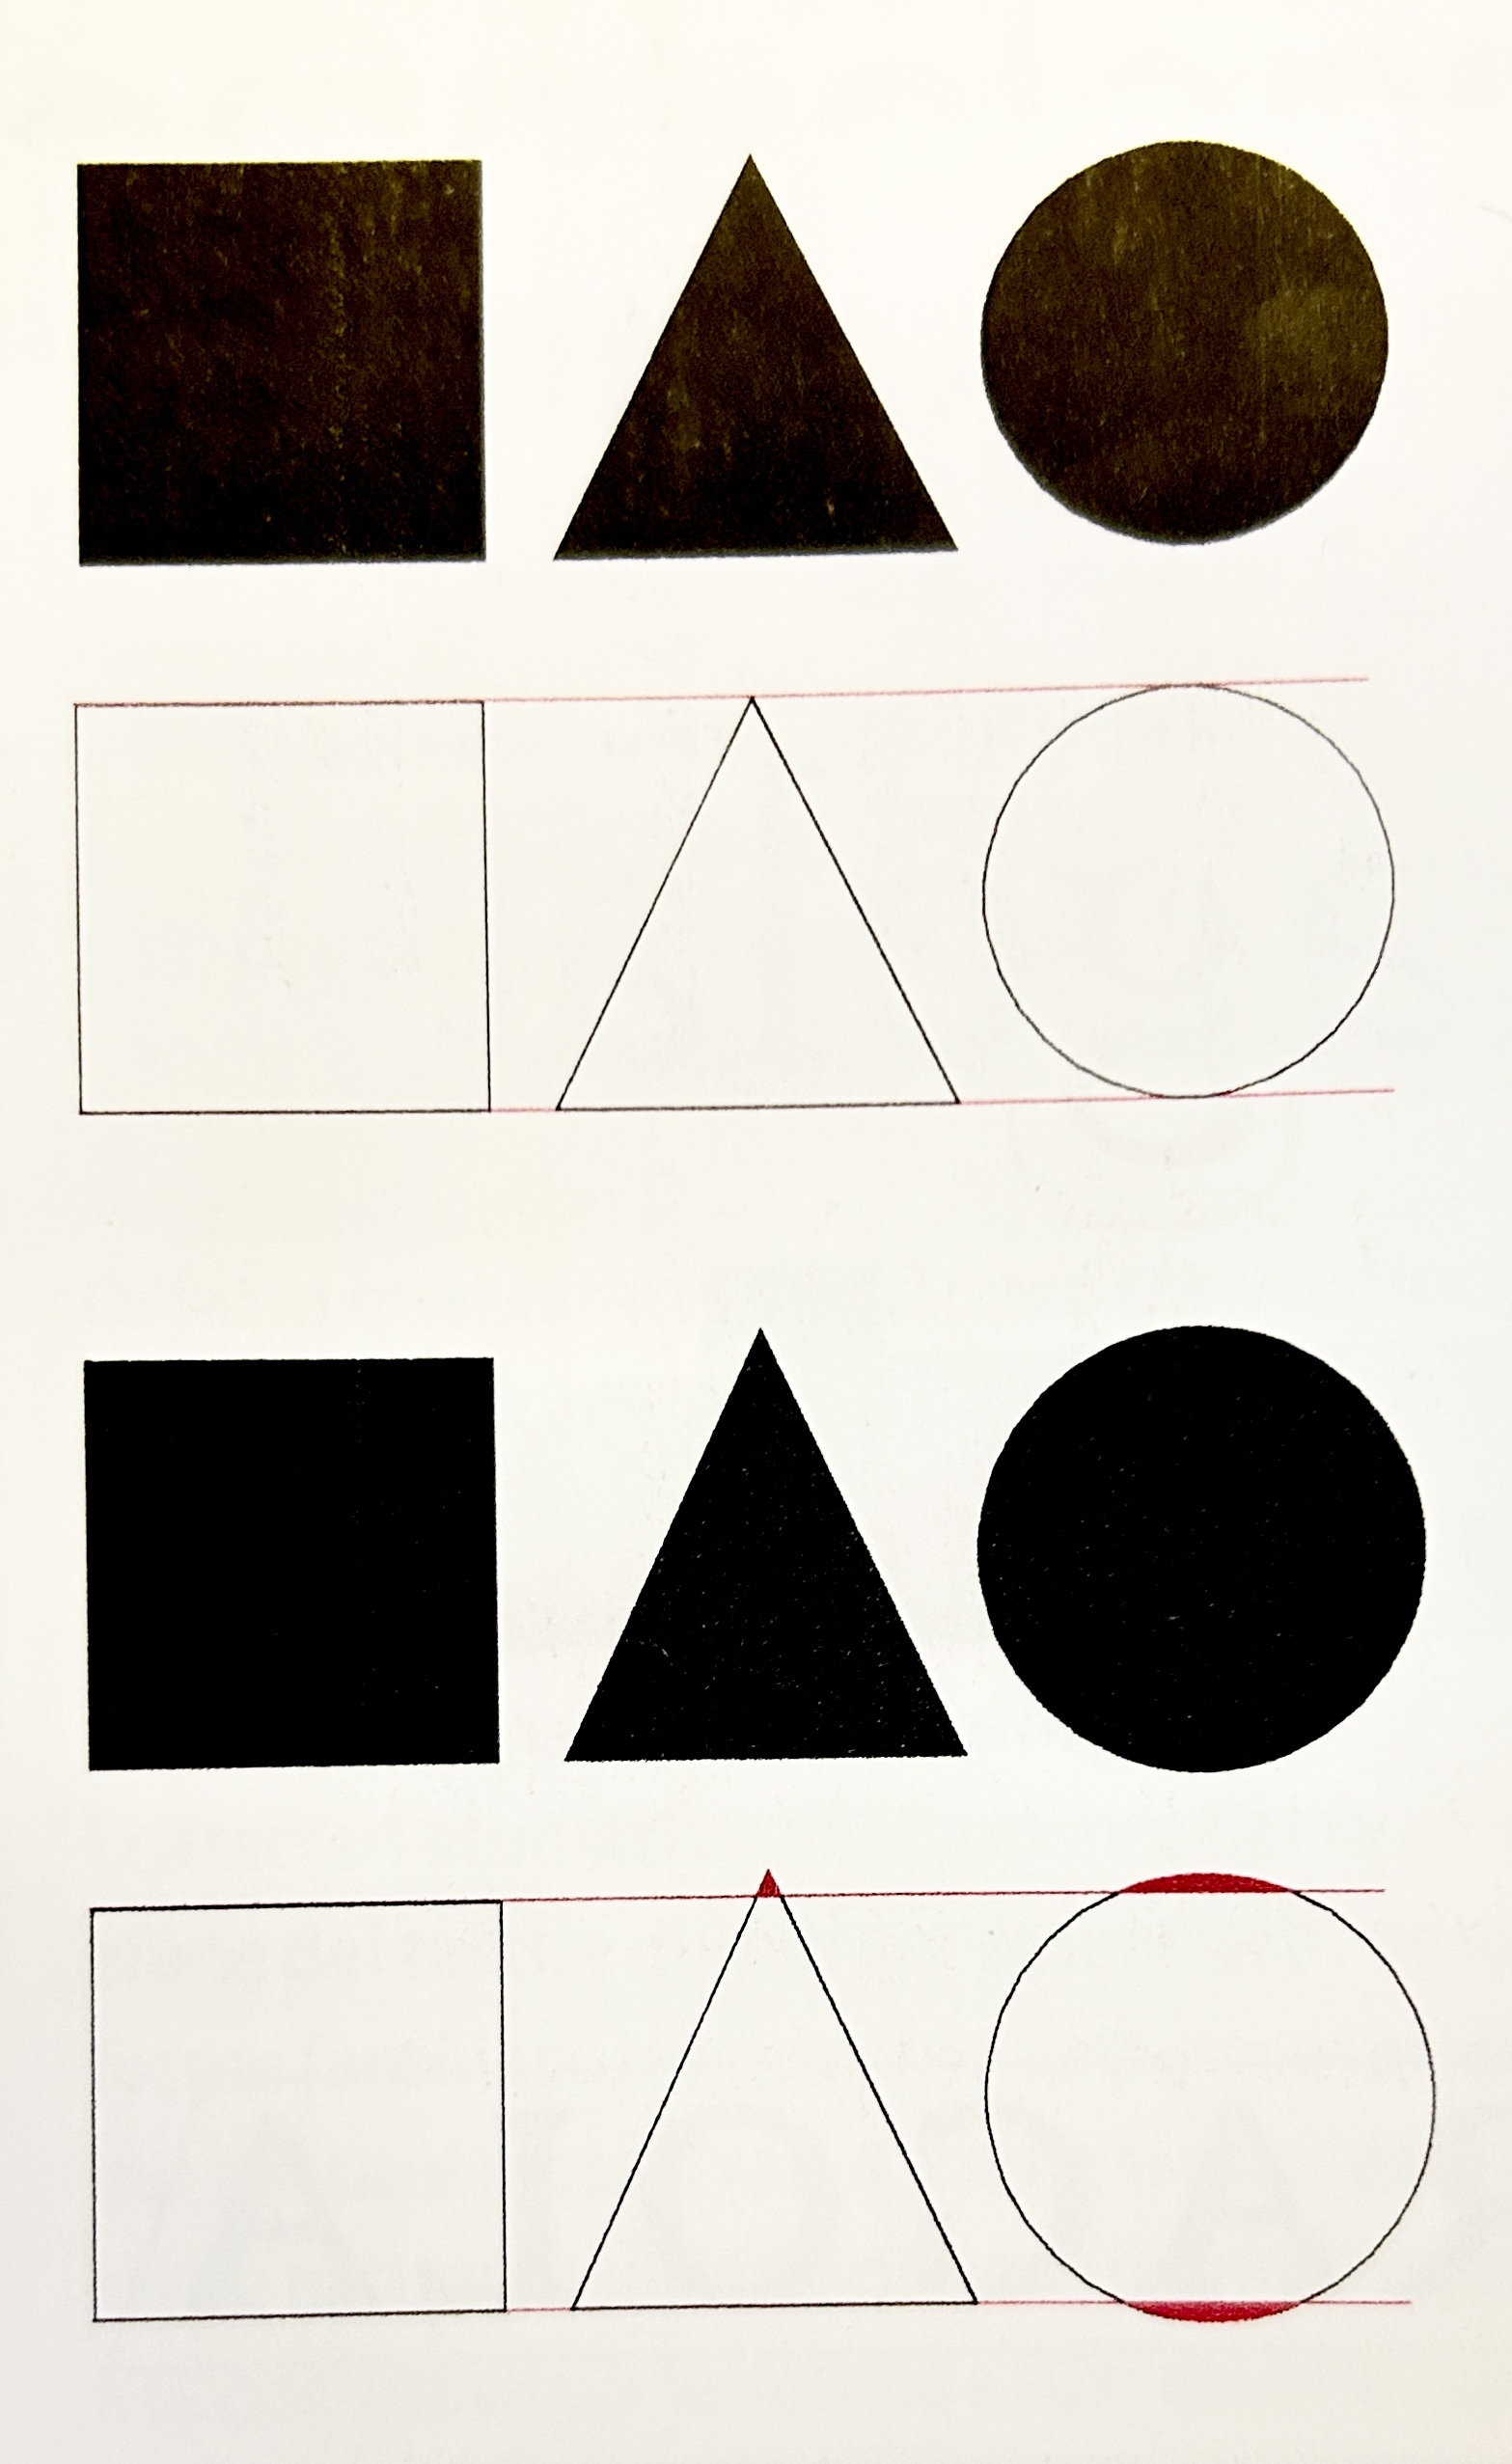
\includegraphics[width=0.3\linewidth]{lezione_2 - correzioni ottiche/imgs/IMG_4754.jpg}
\end{figure}
\begin{mdframed}[style=mystyle,frametitle=Curiosità]
Già i Romani avevano già notato questo effetto ottico! 
\end{mdframed}

\section{Caso 2: centro ottico e geometrico}
Prendendo un piano tagliato orizzontale perfettamente in due metà, la parte superiore viene percepita come più grande rispetto alla sottostante.

Questo accade con lettere come la B, H, E, X, S, K... ed in generale con quelle lettere che presentano barre,bracci e aste 
\\\\
Per risolvere, si discosta il centro geometrico verso l'alto, creando il cosiddetto \hl{centro ottico}, che è al di sopra di quello geometrico di pochi millimetri. In questo modo, l'occhio, vedrà la lettera come uniforme e ben armoniosa

\begin{figure}[H]
    \centering
    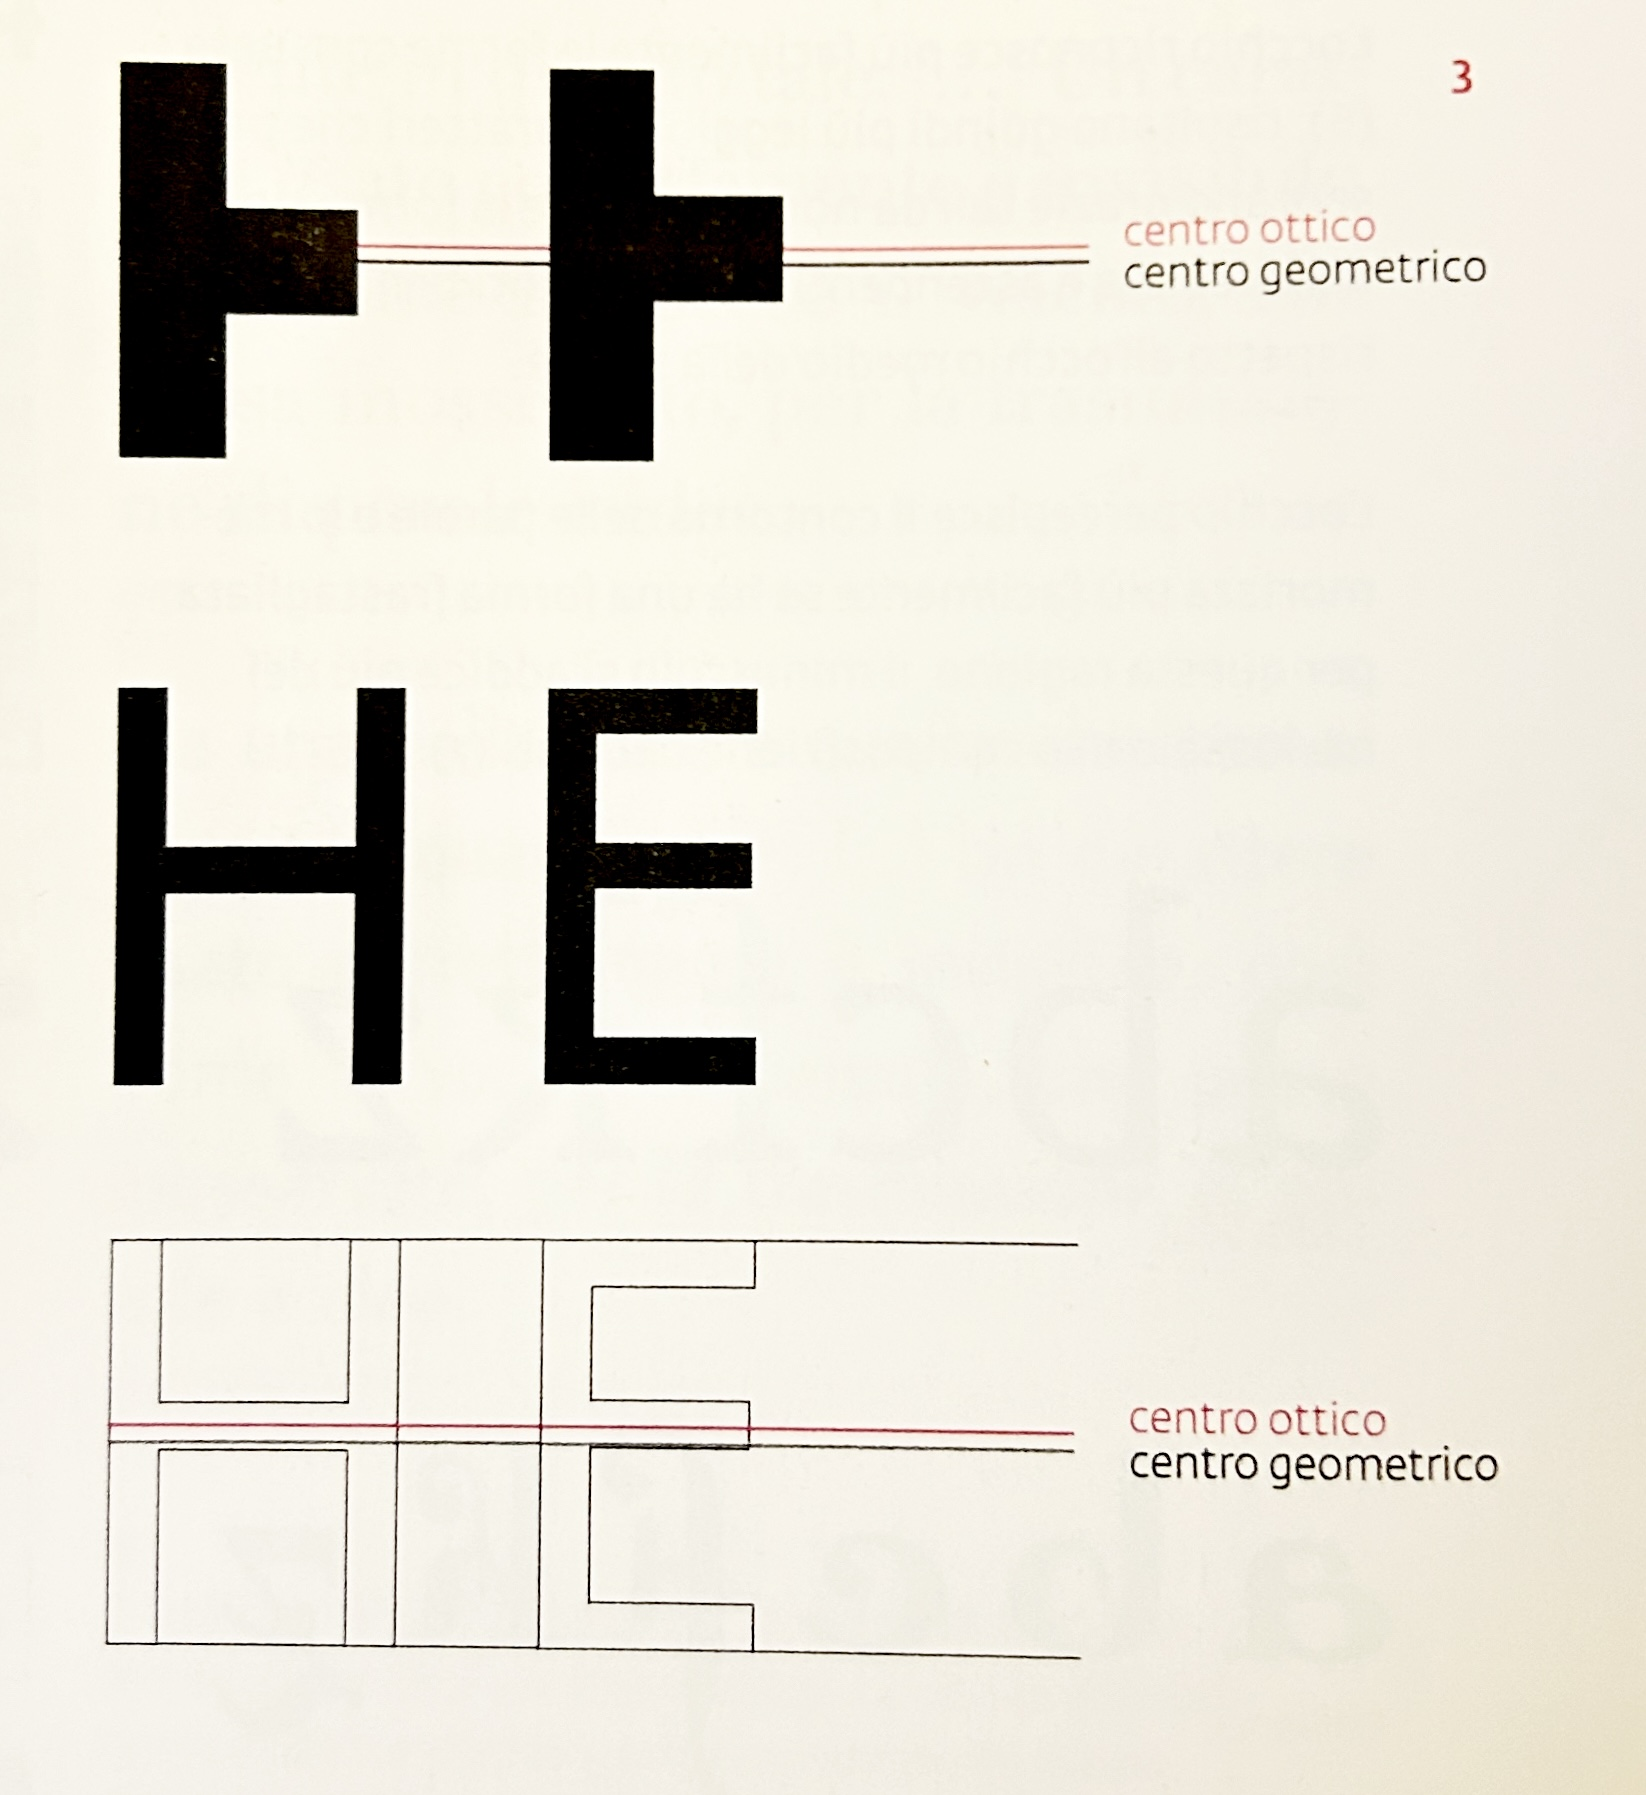
\includegraphics[width=0.3\linewidth]{lezione_2 - correzioni ottiche/imgs/IMG_4755.jpg}
\end{figure}

\section{Caso 3: sovrapposizione di forme}
Caso che vale con molte delle lettere già mostrato nel \textit{\textbf{caso 2}}, questa casistica si basa sul verso di lettura dell'occhio (\hl{l'occhio, infatti, scansiona dall'alto verso il basso}). Partendo da questo presupposto, le lettere composte dalla sovrapposizione di forme uguali/molto simili, presentano una parte superiore che visivamente è più grande di quella inferiore (B, C, G, S, Z, X, K, E).
\\\\
Per risolvere, si effettuano modifiche che variano da lettera a lettera, ma che si basano sul medesimo concetto: aumentare leggermente la dimensione della parte sottostante, e diminuire la parte superiore
\begin{figure}[H]
    \centering
    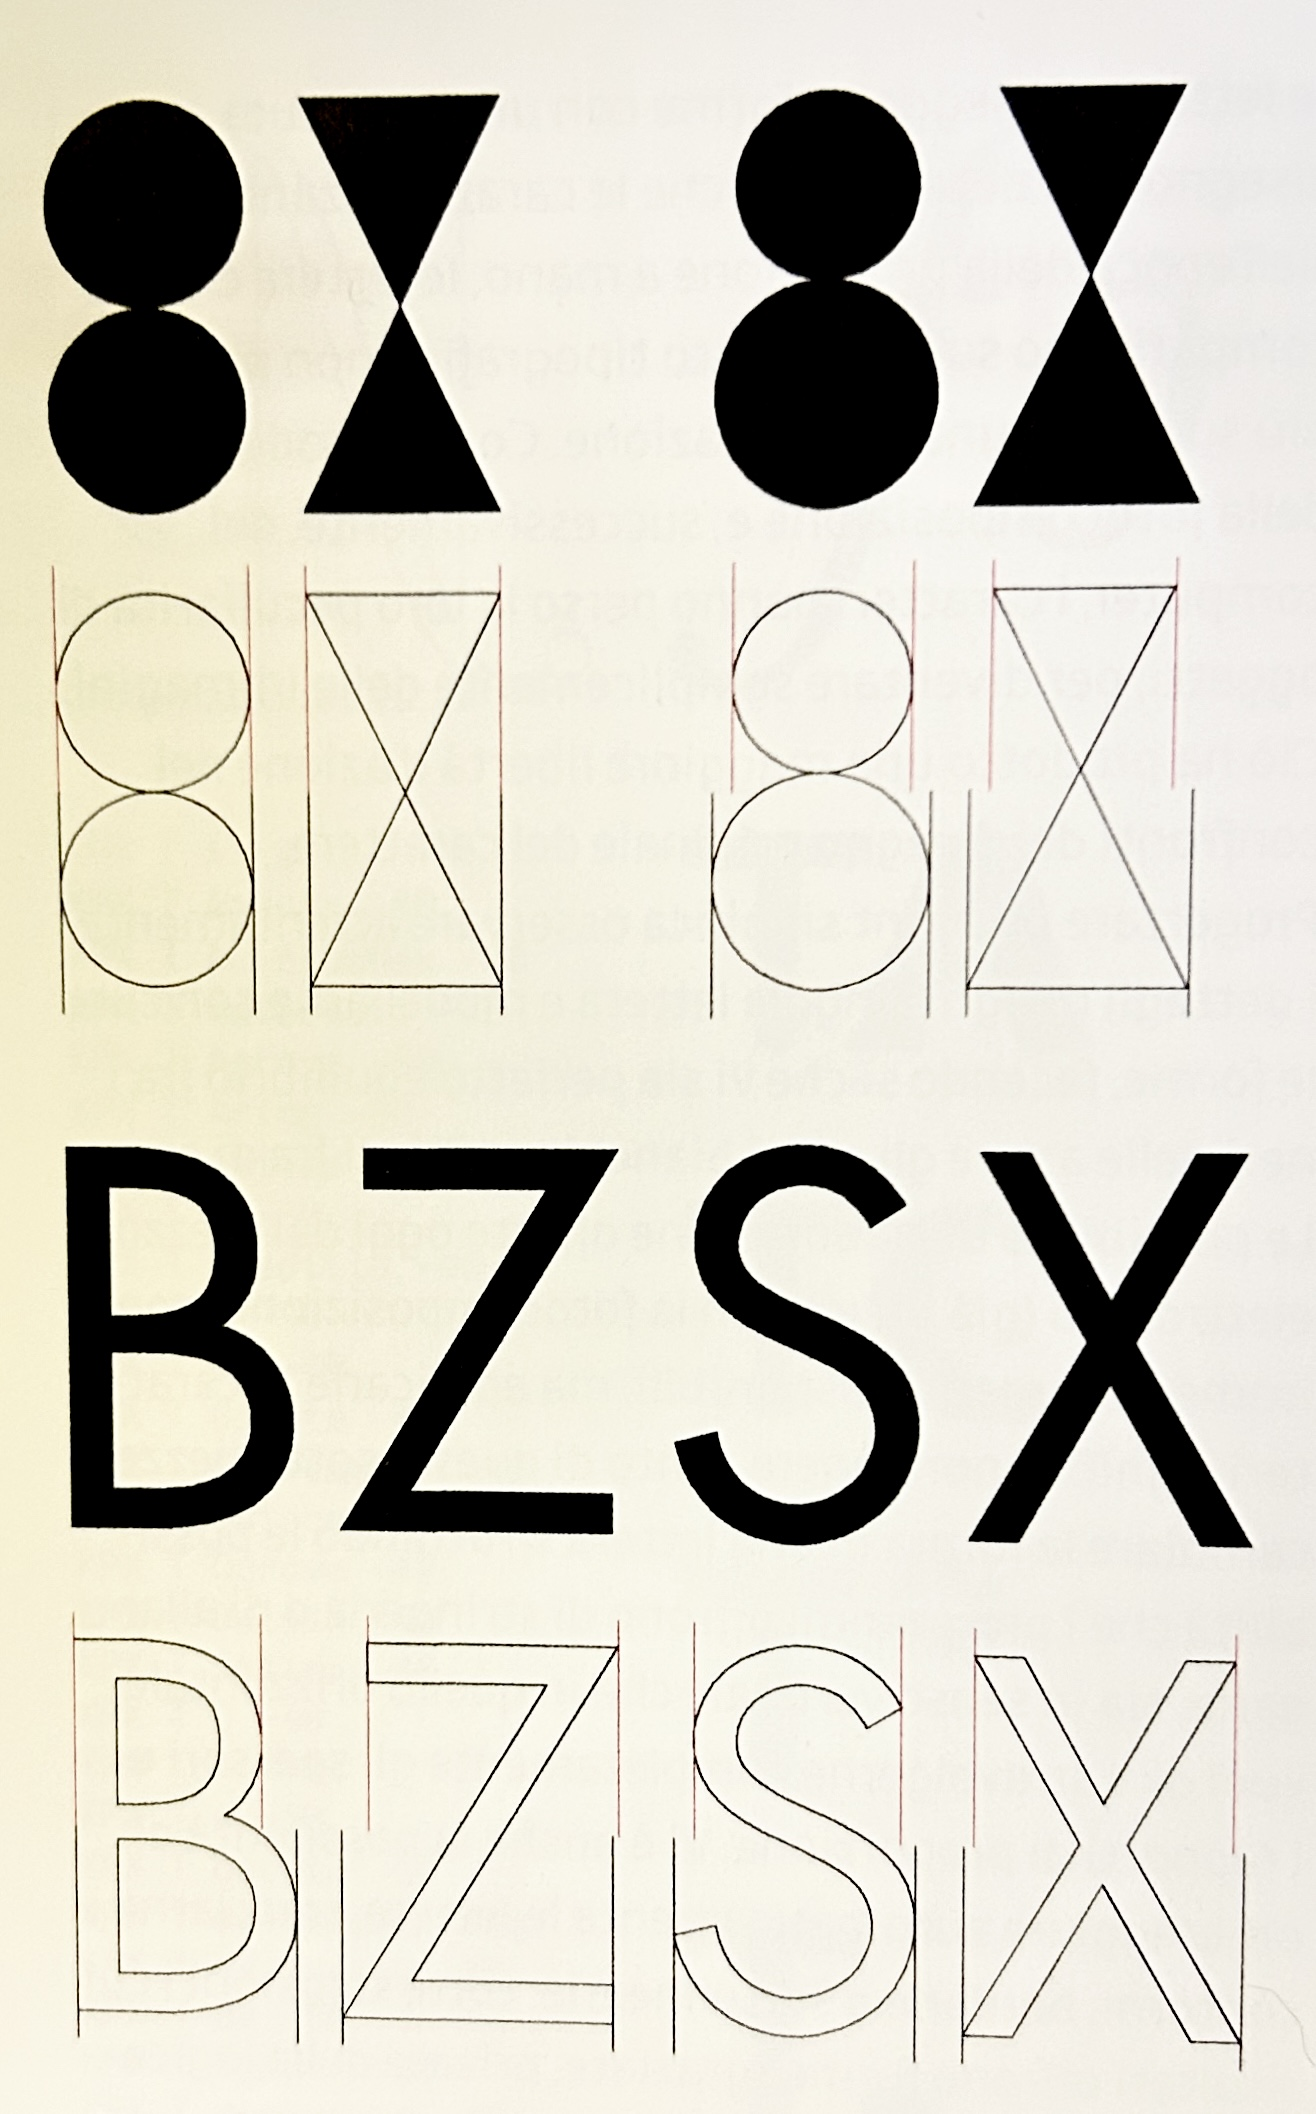
\includegraphics[width=0.3\linewidth]{lezione_2 - correzioni ottiche/imgs/IMG_4758.jpg}
\end{figure}

\section{Caso 4: linee orizzontali e verticali}
Per l'occhio umano, le aste orizzontali delle lettere vengono percepite come più spesse rispetto a quelle verticali. Questo, come già spiegato nel \textit{\textbf{ caso 3}}, succede perchè l'occhio umano scansiona dall'alto verso il basso.

Per risolvere questa distorsione ottica, viene \hl{modulato} lo spessore delle aste orizzontali: si tende a diminuire di qualche punto lo spessore orizzontale.

Lo stesso principio vale per le lettere che presentano curve (questo tipo di correzione viene applicata a lettere come la T, F, E, O...)
\begin{figure}[H]
    \centering
    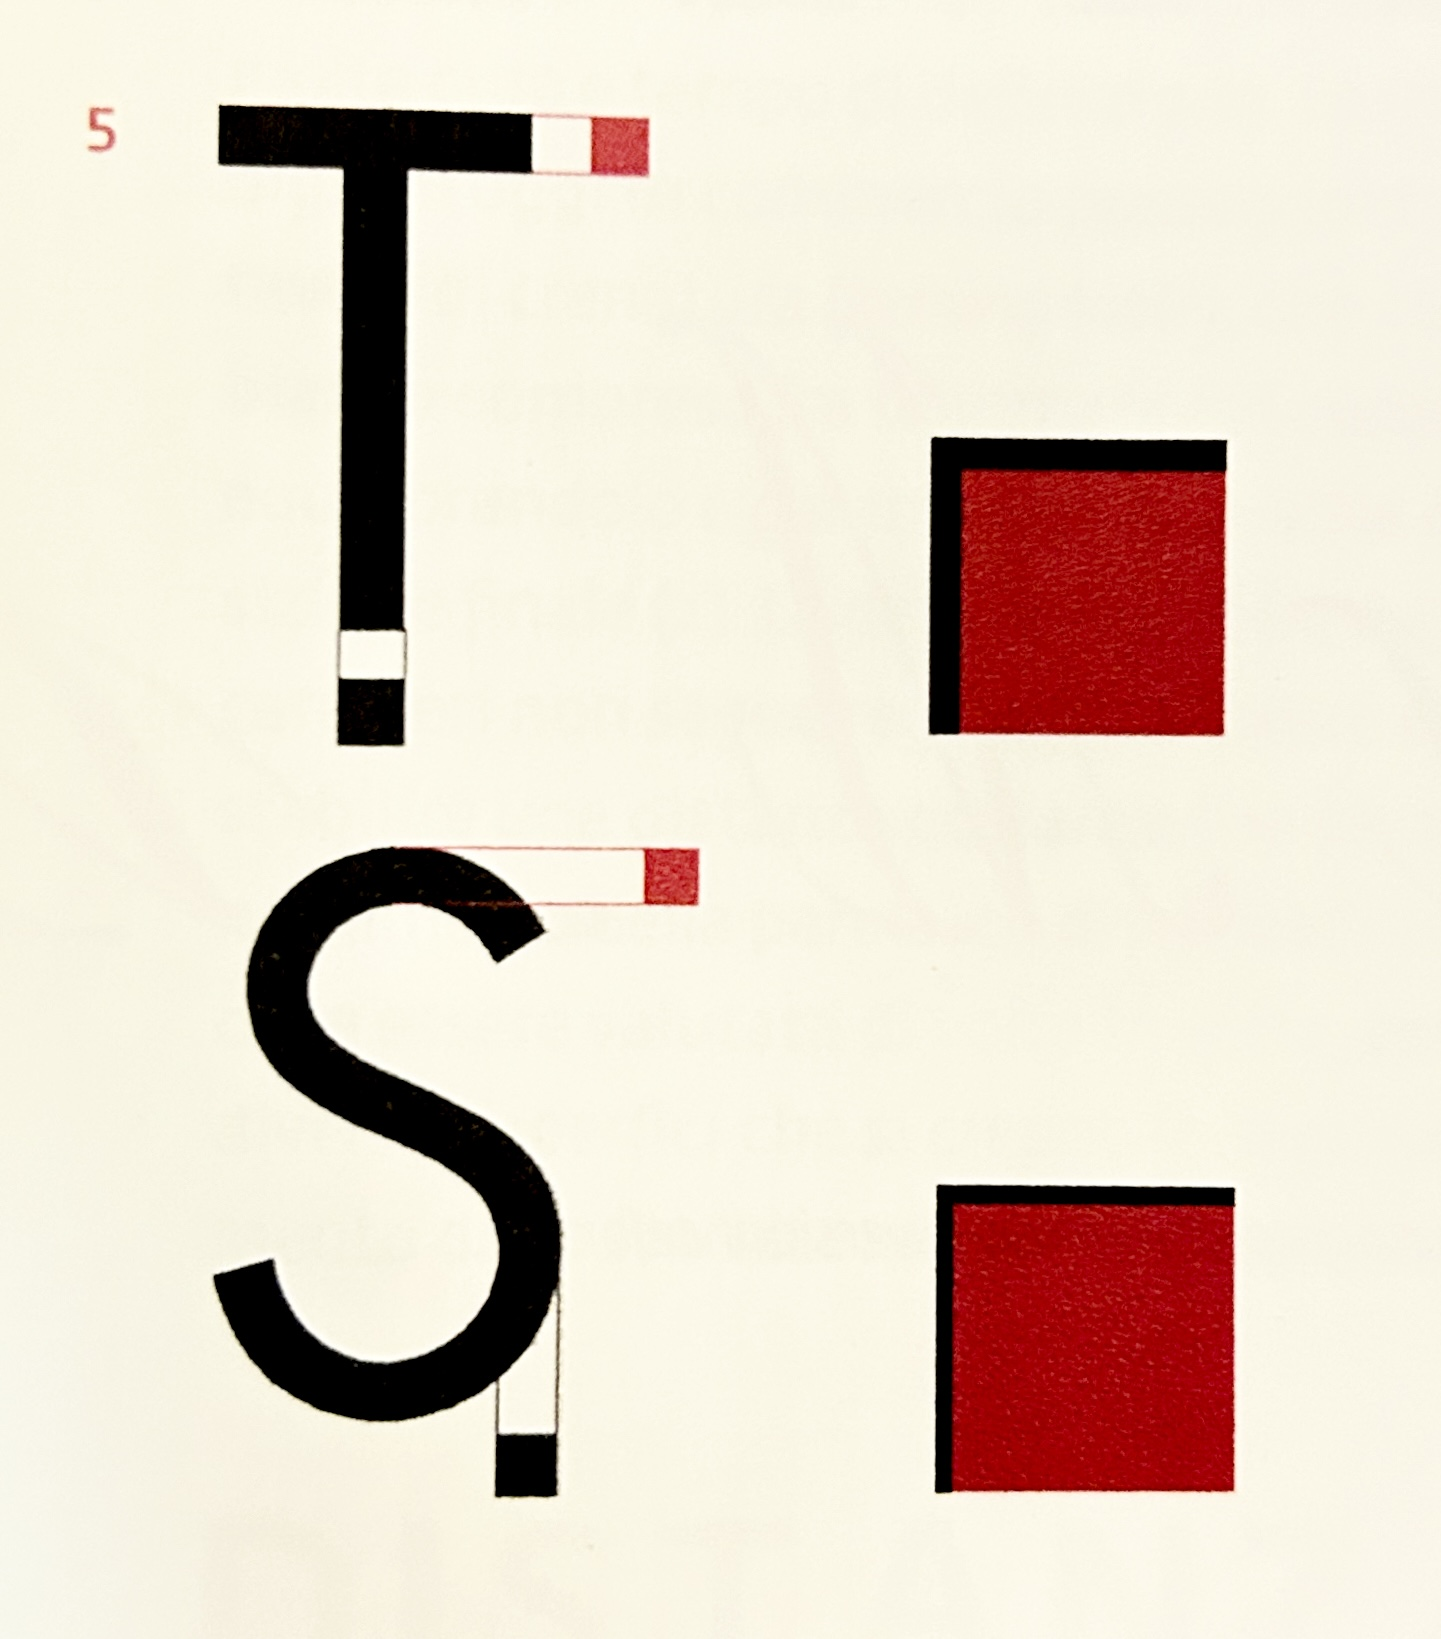
\includegraphics[width=0.3\linewidth]{lezione_2 - correzioni ottiche/imgs/IMG_4757.jpg}
\end{figure}

\section{Caso 5: incontro tra rette, curve e diagonali}
Per i casi che verranno elencati, viene applicato un alleggerimento nel punto di contatto dal momento che l'occhio lo vede come più pesante rispetto al resto della lettera:
\begin{itemize}
    \item incontro retta-curva
    \item incontro curva.curva
    \item incontro diagonale-diagonale
\end{itemize}
questo vale per lettere come la \textit{\textbf{v}} o la \textbf{\textit{a}} minuscola.
\begin{figure}[H]
    \centering
    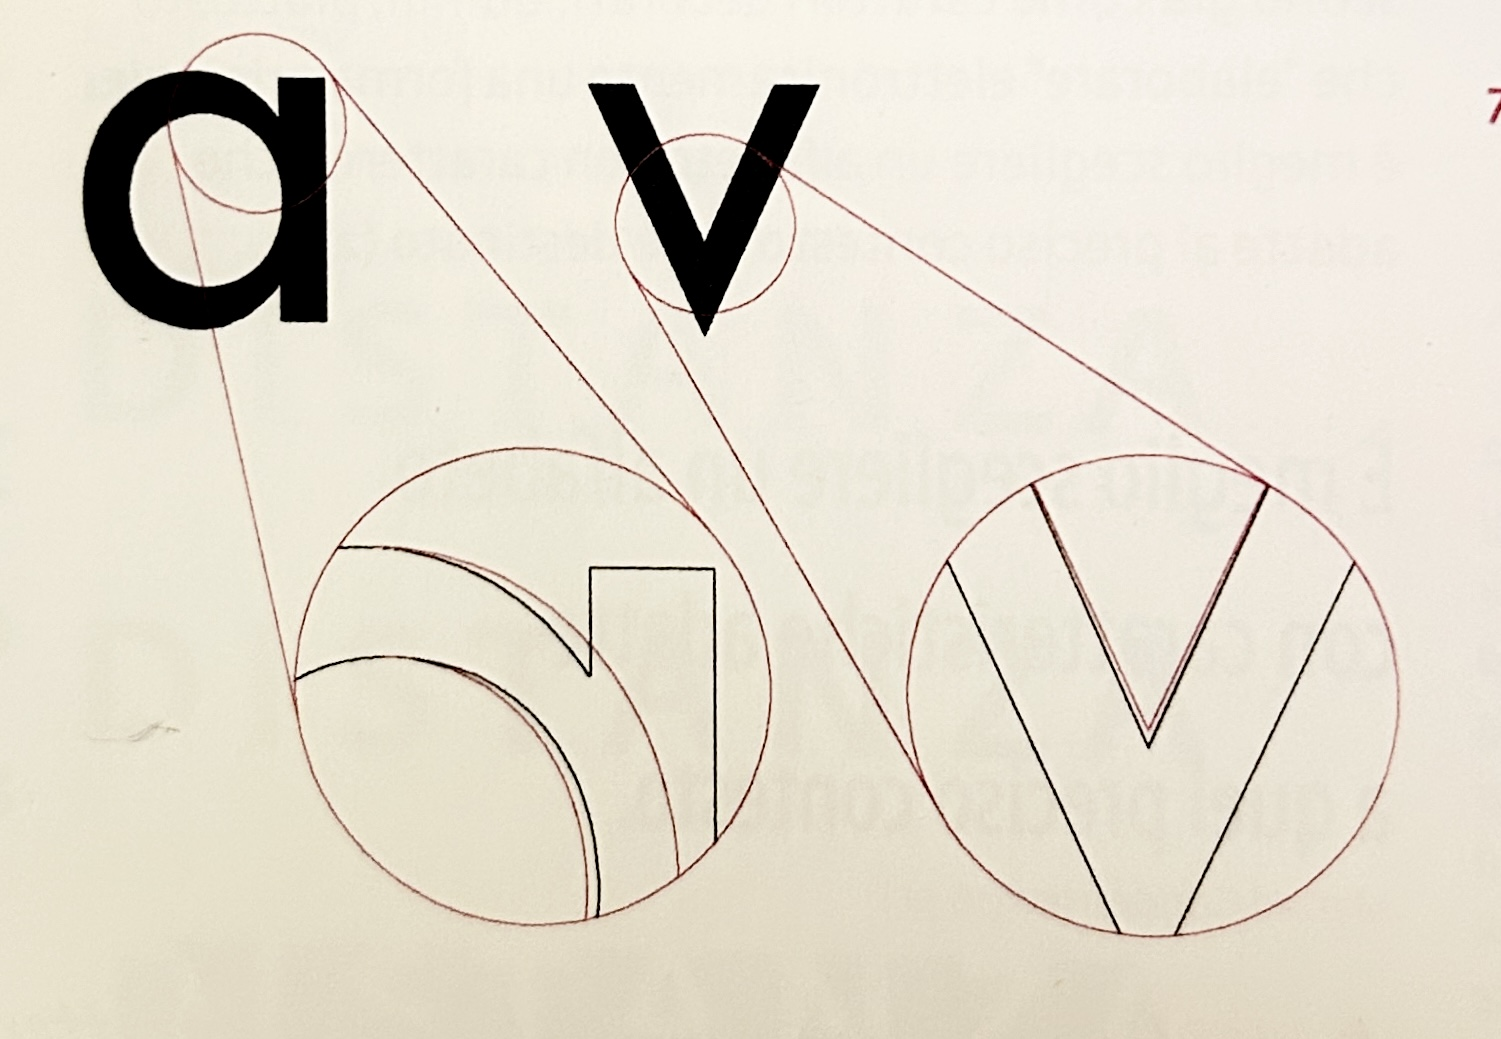
\includegraphics[width=0.3\linewidth]{lezione_2 - correzioni ottiche/imgs/IMG_4759.jpg}
\end{figure}


